\section{Versuchsaufbau/-durchführung}

Bei den Teilversuchen \emph{Zeitabhängigkeit der Schwingungsamplitude}
und \emph{Widerstandsbestimmung für den ap. Grenzfall} wird der selbe
Versuchsaufbau \ref{fig:aufbau_eins} verwendet. Lediglich der Widerstand ist bei dem
zweiten Teilversuch variabel einstellbar.
\begin{figure}
  \centering
  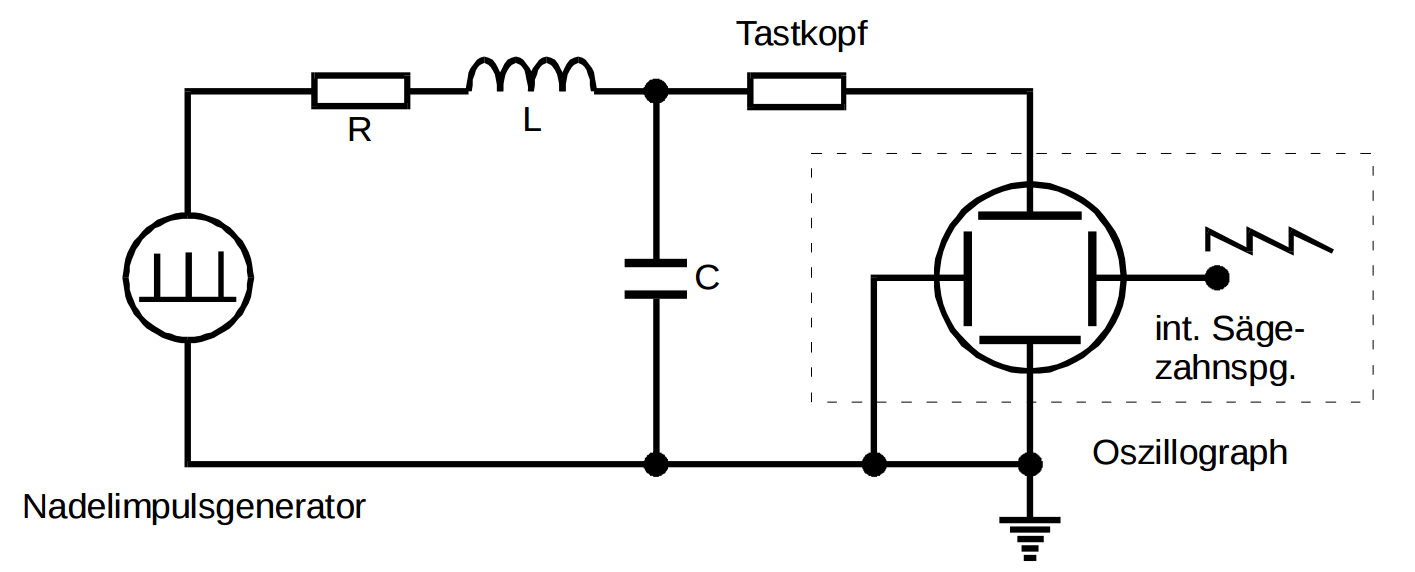
\includegraphics[width = 0.5\textwidth]{bilder/erster_versuchsaufbau.png}
  \caption{Versuchsaufbau für die Untersuchung der Schwingungsamplitude und des ap. Grenzfalles \cite{anleitung354}. }
  \label{fig:aufbau_eins}
\end{figure}


\subsection{Zeitabhängigkeit der Schwingungsamplitude}

Am Anfang muss die Frequenz des Generator
so eingestellt werden, dass die Kondensatorspannung um den Faktor $3$ bis $8$
abgenommen hat. Mithilfe der 'Cursor'-Funktion des Oszilloskops, wird dann
die Höhe von allen oberen Schwingungsbäuchen gemessen.

\subsection{Widerstandsbestimmung für den ap. Grenzfall}

Für die Bestimmung des Wiederstandes an dem sich
der aperiodische Grenzfall befindet, wird das Potentiometer
auf seinen Maximalwert eingestellt.
Der Widerstand wird nun kontinuierlich verringt, dabei wird das
Ozsilloskop beobachtet. Man dreht den Widerstand soweit runter, bis
ein Überschwinger ($\frac{\map{d}U\ua{C}}{\map{d}t}>0$) entdeckt wird.
Der Wiederstand wird nun soweit erhöht, bis der Überschwinger gerade verschwindet.
An dieser Stelle befindest sich der ap. Grenzfall und somit $R\ua{ap}$.

\subsection{Frequenzabhängigkeit der Kondensatorspannung und Phase}
\begin{figure}
  \centering
  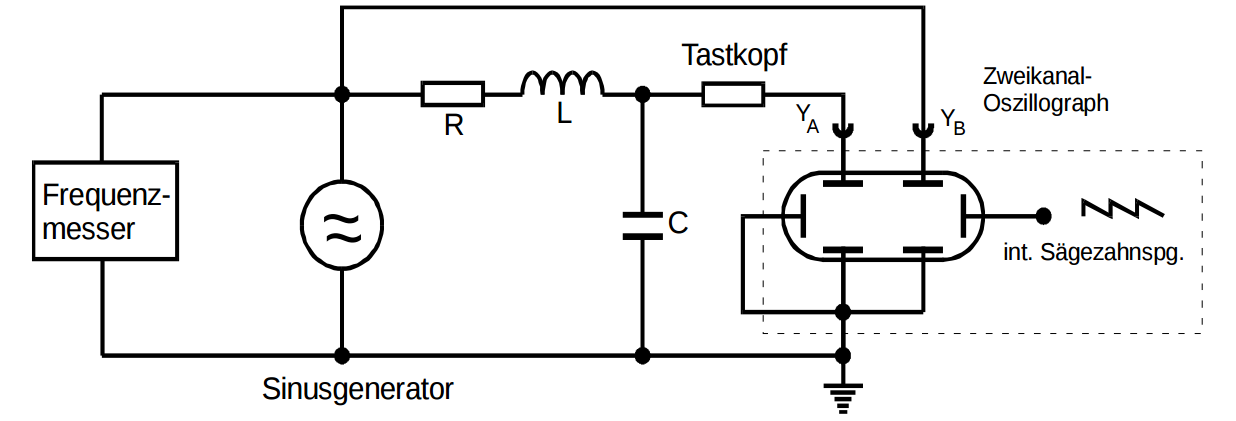
\includegraphics[width = 0.5\textwidth]{bilder/aufbau_zwei.png}
  \caption{Versuchsaufbau für die Untersuchung der Frequenzabhängigkeit der Kondensatorspannung und Phase \cite{anleitung354}. }
  \label{fig:aufbau_zwei}
\end{figure}


Der Versuch wird nach Abbildung \ref{fig:aufbau_zwei} aufgebaut.
Die am Generator anliegende Frequenz wird im Intervall $f\in\left[25,45\right]\,\si{\kilo\hertz}$
varriiert. Mithilfe der 'Measure'-Funktion des Ozsillsokops
kann Generator- und Kondensatorspannung bei verschieden Frequenzen
abgelesen werden. Zusätzlich wird mit ihr die Phasenlänge $b$ der Generatorspannung
gemessen. Abschließend bietet die 'Cursor'-Funktion eine Möglichkeit, um
die zeitliche Differenz $a$ zwischen Generator- und Kondensatorspannung zu
bestimmen.
Mit den Größen $a$ und $b$ kann dann der Phasenunterschied zwischen
Generator- und Kondensatorspannung errechnet werden:

\begin{equation}
  \label{eq:phasen_unterschied}
  \varphi=\frac{2a}{b}\pi.
\end{equation}
